% ============================================================================
%  Chapter 5. Weak Supervision and the Inherited Prior
%
%  \input file. Requires booktabs, amsmath, natbib in the parent preamble.
%  Bibliography: accord/thesis/refs.bib
%
%  Traceability: accord/CORRECTIONS.md (C9), the weak-labelling run logs, and
%  the per-rule predicted-positive rates recorded in the audit outputs.
% ============================================================================

\chapter{Weak Supervision and the Inherited Prior}
\label{ch:weak}

\section{The Question This Chapter Answers}
\label{sec:weak-overview}

Chapter~\ref{ch:candidates} produced $1{,}978$ candidate pairs and, for $299$ of
them, a pharmacist's judgement. Training a supervised detector on $299$
annotations containing $12$ positives is not viable. The standard remedy is weak
supervision: obtain approximate labels cheaply for the remaining pool, accept
that they are noisy, and rely on the model to average over the noise
\citep{ratner2017snorkel}. Since 2023 the dominant cheap labeller has been an
instruction-tuned language model, on the strength of results showing that such
models match or exceed crowd annotators on several classification tasks
\citep{gilardi2023chatgpt}.

This chapter reports what happened when that recipe was applied to
cross-note medication contradiction detection, and it is the clearest example in
this thesis of a failure that is entirely diagnosable in advance and was not
diagnosed.

\paragraph{Research question.} Can an instruction-tuned open-weights language
model supply usable weak labels for a rare, clinically technical, pairwise
judgement, in a regime where the true positive rate is around $4\%$?

\paragraph{Answer.} No, and the failure is not one of accuracy on individual
examples. It is a failure of \emph{prior}. The labeller assigned the positive
class to $84.9\%$ of candidates against a pharmacist-measured base rate of
$4.0\%$, a prevalence mismatch of roughly $21\times$. The detector trained on
those labels reproduced the labeller's per-rule positive rate almost exactly,
which is the behaviour of a student that has learned its teacher's marginal and
nothing about the input.

\section{Setup}
\label{sec:weak-setup}

\subsection{Labeller and pool}

The weak labeller is Llama 3 8B \citep{grattafiori2024llama3}, run locally. It
was presented with each candidate's exemplar pair, the nursing sentence and the
discharge sentence, together with the rule that generated the candidate, and
asked for a binary judgement: \emph{contradiction} or \emph{not\_contradiction},
plus a confidence value.

The labelled pool is $1{,}679$ rows. This is exactly the $1{,}978$ candidates of
Chapter~\ref{ch:candidates} minus the $299$ pairs sent to the pharmacist, so the
weak-label training set and the gold evaluation set are disjoint by
construction. That part of the design is correct and is worth stating, because
much else in this chapter is not.

\subsection{What the labeller was shown}

The labeller saw the exemplar sentence pair. Chapter~\ref{ch:candidates},
Section~\ref{sec:exemplar}, established that for $41.4\%$ of action-conflict
candidates the exemplar pair did not carry the conflict that triggered the
candidate, while the prompt asserted, via the rule identifier, that a conflict
of that type was present. The labeller was therefore told, for a large minority
of rows, that a conflict existed in a sentence pair that did not exhibit one.
Section~\ref{sec:weak-acquiescence} argues that this is one of several mutually
reinforcing pressures towards the positive class, and that the design contained
no mechanism for any of them to be detected.

\section{The Prevalence Mismatch}
\label{sec:weak-prevalence}

\begin{table}[t]
\centering
\small
\begin{tabular}{lrr}
\toprule
 & \textbf{Count} & \textbf{Rate} \\
\midrule
Weak label $=$ \emph{contradiction}      & 1,425 & 84.9\% \\
Weak label $=$ \emph{not\_contradiction} & 254   & 15.1\% \\
\midrule
Total labelled                            & 1,679 & \\
\midrule
Pharmacist base rate (gold, $n{=}299$)    & 12 & 4.0\% \\
\midrule
\textbf{Prevalence ratio}                 & & \textbf{$\approx 21\times$} \\
\bottomrule
\end{tabular}
\caption{The weak labeller's marginal against the measured base rate. The
labeller assigns the positive class at roughly twenty-one times the rate a
board-certified pharmacist does. This is the single number that determines
everything the trained model subsequently does.}
\label{tab:prevalence}
\end{table}

Table~\ref{tab:prevalence} is the chapter's central result. Two derivations make
its severity concrete. Both are arithmetic from the reported counts and are
labelled as derived.

\paragraph{Derivation 1: the floor on false positives.} If the pharmacist's
$4.0\%$ base rate holds in the unlabelled pool, then approximately $67$ of the
$1{,}679$ rows are true contradictions. The labeller calls $1{,}425$ of them
positive. Even granting the labeller perfect recall, at least
$1{,}425 - 67 = 1{,}358$ of its positive labels are wrong. More than $95\%$ of
the positive supervision signal is noise, and it is not symmetric noise: it is
concentrated entirely in one class.

\paragraph{Derivation 2: the label is nearly constant.} A label that takes one
value $84.9\%$ of the time carries little information about the input regardless
of how it is distributed. Under this supervision, the loss-minimising strategy
for a model with sufficient capacity to fit the marginal but insufficient signal
to fit the conditional is to predict the majority class with high confidence.
Section~\ref{sec:weak-tracking} shows that this is what happened.

\paragraph{Why standard weak-supervision theory does not rescue this.}
Aggregation frameworks such as Snorkel \citep{ratner2017snorkel} are designed for
noise that is \emph{conditionally independent across sources given the true
label}, and their guarantees rest on having multiple sources whose errors are
not aligned. Here there is one source. Its error is a systematic prior shift, not
independent noise, and no amount of downstream averaging removes a shifted
marginal. The recipe was applied outside the regime in which it works.

\section{The Student Inherits the Teacher's Marginal}
\label{sec:weak-tracking}

\begin{table}[t]
\centering
\small
\begin{tabular}{clrrr}
\toprule
\textbf{Rule} & \textbf{Trigger} & \textbf{Llama} & \textbf{ACCORD} & \textbf{True} \\
              &                  & \textbf{pos.\ rate} & \textbf{pos.\ rate} & \textbf{prevalence} \\
\midrule
1 & Direct action conflict & 95.5\% & 97.0\% & 2.2\% \\
2 & Drug class conflict    & 96.8\% & 96.8\% & 9.7\% \\
3 & Dosage conflict        & 98.7\% & 97.5\% & 5.1\% \\
4 & Omission               & 45.5\% & 74.5\% & 3.6\% \\
\bottomrule
\end{tabular}
\caption{Predicted-positive rates by rule. ``Llama pos.\ rate'' is the fraction
of that rule's candidates the weak labeller called a contradiction; ``ACCORD
pos.\ rate'' is the fraction the trained detector predicts positive at threshold
$0.5$; ``true prevalence'' is the pharmacist-measured rate from
Table~\ref{tab:gold}. On Rules 1 to 3 the student tracks the teacher to within
$1.5$ percentage points while both sit an order of magnitude above the truth.
Rule 4 is the exception, and the direction of the exception is diagnostic:
ACCORD does not reproduce the teacher's selectivity, it regresses towards its
own global positive prior.}
\label{tab:tracking}
\end{table}

Table~\ref{tab:tracking} is the mechanism behind Chapter~\ref{ch:eval}'s
results. Three readings.

\paragraph{Rules 1 to 3: near-perfect marginal transfer.} The student's positive
rate differs from the teacher's by $1.5$, $0.0$, and $1.2$ percentage points.
Meanwhile the true prevalence varies by more than a factor of four across those
same three rules ($2.2\%$, $9.7\%$, $5.1\%$). The student reproduces the
quantity that carries no information about the truth and does not reproduce the
quantity that does. This is not a model that learned a noisy version of the
task. It is a model that learned the label's marginal distribution.

\paragraph{Rule 4: the teacher's one real distinction, discarded.} The weak
labeller behaves visibly differently on Rule 4, calling only $45.5\%$ of
omission candidates positive against $95\%$ to $99\%$ elsewhere. There is a plain
explanation: Rule 4 candidates have an \emph{empty} discharge side, since the
drug is absent from the discharge summary by construction. Presented with a
sentence and nothing to compare it to, the labeller declines roughly half the
time. Whether this reflects clinical reasoning or a formatting response to a
degenerate input cannot be determined from the labels alone, and the distinction
matters: the true prevalence on Rule 4 is $3.6\%$, so even at $45.5\%$ the
labeller is still more than twelve times too positive.

What the student does with this is the informative part. ACCORD's Rule 4
positive rate is $74.5\%$, roughly midway between the teacher's $45.5\%$ and its
own global rate. The one place where the supervision carried a real
input-dependent signal is the one place where the student partially discarded
it, pulling towards its majority prior. A model learning the conditional would
have sharpened the distinction; a model learning the marginal blunts it.

\paragraph{The consequence for precision.} If a detector predicts positive at
rate $p$ on a subpopulation whose true prevalence is $\pi$, and its predictions
are independent of the label, its precision is $\pi / p \cdot p = \pi$ in
expectation, that is, exactly the base rate. Table~\ref{tab:gold} in
Chapter~\ref{ch:candidates} shows precisely this: $2.3$ against $2.2$, $10.0$
against $9.7$, $5.2$ against $5.1$. The apparent variation in ACCORD's precision
across rules is entirely explained by variation in the rules' own base rates.

\section{The Degenerate Confidence Field}
\label{sec:weak-confidence}

\subsection{The finding}

The weak labelling produced a \texttt{weak\_confidence} field alongside each
label. Across all $1{,}679$ training rows and all $299$ audit rows it takes
exactly two values:
\[
\texttt{weak\_confidence} =
\begin{cases}
0.95 & \text{iff } \texttt{weak\_label} = \textit{contradiction},\\
1.00 & \text{iff } \texttt{weak\_label} = \textit{not\_contradiction}.
\end{cases}
\]
It is a deterministic function of the label. It contains no information about
the labeller's uncertainty on any individual example, and it cannot, because it
does not vary within a label class.

\subsection{Why this is worse than a useless field}

An unused useless field is harmless. This one was used, in two places, both of
which convert a label into a training-time intervention.

\paragraph{As a filter.} The training code discards rows with
$\texttt{weak\_confidence} < 0.9$. Since the field's minimum value is $0.95$,
this filter removes nothing. It is a no-op that reads, in the code and in every
description of the pipeline, as a quality-control step. Its presence created the
appearance of confidence-based data cleaning where none occurred.

\paragraph{As a loss weight.} The same field is multiplied into the per-example
loss. Because the field is a function of the label, this is a
\emph{label-conditioned reweighting}: every positive example's loss is scaled by
$0.95$ and every negative's by $1.00$. The direction is perverse. The positive
class is already the overwhelming majority at $84.9\%$, and the reweighting
further downweights it by $5\%$ relative to the minority class, which is a
five-percent nudge in the right direction applied to a twenty-one-fold error in
the wrong one. The magnitude is negligible; the fact that the pipeline contained
a label-dependent loss weight that nobody intended is not.

\subsection{The general lesson}

A confidence field emitted by a language model alongside a label is not a
calibrated probability and should not be treated as one without measurement
\citep{guo2017calibration,zhao2021calibrate}. The specific diagnostic that
would have caught this is trivial and should be mandatory: \emph{print the
number of distinct values a confidence field takes, and its conditional
distribution given the label, before using it for anything}. Two distinct
values, perfectly separated by label, is a result that takes one line of code to
obtain and ends the discussion.

\section{Why the Labeller Says Yes}
\label{sec:weak-acquiescence}

The chapter has established that the labeller is systematically positive. It is
worth separating the candidate explanations, because they have different
remedies and because this thesis is not in a position to adjudicate between
them.

\paragraph{The prompt asserts the conclusion.} Each candidate was presented
together with the rule that produced it, which names a conflict type. A prompt
that says ``this pair was flagged as a direct action conflict; is it a
contradiction?'' contains its own answer. This is the most likely dominant
cause and the cheapest to test.

\paragraph{The evidence frequently does not support the assertion.} For $41.4\%$
of action-conflict candidates the exemplar pair did not carry the conflict
(Chapter~\ref{ch:candidates}). A labeller that resolves the tension between a
confident framing and unsupportive evidence in favour of the framing will be
systematically positive, and will be so most often exactly where the evidence is
weakest.

\paragraph{Class-prior insensitivity.} Instruction-tuned models are known to
carry strong, prompt-sensitive class priors that do not track the true base rate
of the task \citep{zhao2021calibrate}. A task with a $4\%$ positive rate is far
outside the regime where an unanchored prior is harmless.

\paragraph{Failure defaults.} A related component of this project scored every
unparseable generation and every exception as a positive prediction, which
inflates the positive rate mechanically. [TODO: determine whether the
contradiction weak-labelling loop used the same failure default. If it did, some
unknown share of the $1{,}425$ positives are parse failures rather than
judgements, and the $84.9\%$ figure decomposes into a judgement rate and an
error rate that were never separated.]

\paragraph{What none of these explanations is.} They are not ``the model is bad
at clinical reasoning.'' Chapter~\ref{ch:eval} reports that this same labeller
recovers $11$ of the $12$ true contradictions in the gold set. Its recall is
high. Its problem is entirely that it also says yes to almost everything else,
which is a calibration failure rather than a comprehension failure, and it is
invisible to any evaluation that does not measure the marginal.

\section{What Would Have Caught It}
\label{sec:weak-diagnostics}

The failure in this chapter is fully detectable before any model is trained, at
a cost of a few hours. The following protocol is the constructive contribution
of the chapter and is stated as a general recommendation for LLM weak
supervision on rare-class clinical tasks.

\begin{enumerate}
\item \textbf{Estimate the base rate first, on a small human-labelled sample,
      before generating any weak labels.} A stratified sample of $50$ to $100$
      pairs is enough to establish that the positive rate is single-digit.
      This project produced the pharmacist annotations \emph{after} the weak
      labels, which inverted the only ordering in which the mismatch would have
      been actionable.
\item \textbf{Report the weak labeller's marginal against that base rate, as a
      ratio, before training.} A single printed line, $84.9\%$ against $4.0\%$,
      is a stop condition.
\item \textbf{Report the number of distinct values every confidence field takes,
      and its distribution conditional on the label.}
\item \textbf{Measure the weak labeller against the human labels directly.}
      \citet{pangakis2023validation} argue that any automated annotation
      procedure must be validated against human labels on the same items; this
      project had $299$ such items available and did not compute the
      comparison directly until this audit. Measured against the weak
      labeller's own calls on the $253$ non-ambiguous pairs, Matthews
      correlation is $+0.024$ (TP~$11$, FN~$1$, FP~$212$, TN~$29$), with a
      $95\%$ bootstrap interval of $[-0.1040, +0.0966]$ --- indistinguishable
      from chance, not worse than it. [Correction note: an
      earlier draft cited $-0.044$ here, quoting Chapter~\ref{ch:eval}'s
      system-comparison table; that number belongs to a separately prompted
      Llama 3\,8B evaluation run, not to the weak labeller's own labels, and
      the two must not be conflated.]
\item \textbf{Ablate the rule identifier out of the prompt.} If the positive
      rate moves materially, the prompt was asserting its own conclusion.
      [TODO: run this ablation. It is cheap and it would separate the
      prompt-assertion hypothesis from the class-prior hypothesis.]
\item \textbf{Compare the student's per-rule predicted-positive rate against the
      teacher's.} Table~\ref{tab:tracking} is the diagnostic. Near-identical
      rates across strata whose true prevalences differ by a factor of four is
      the signature of marginal transfer.
\end{enumerate}

None of these is novel as a technique. All of them are omitted routinely,
including here, and the cost of omitting them was the entire supervised half of
this project.

\section{Proposed Figures}
\label{sec:weak-figures}

\begin{figure}[t]
\centering
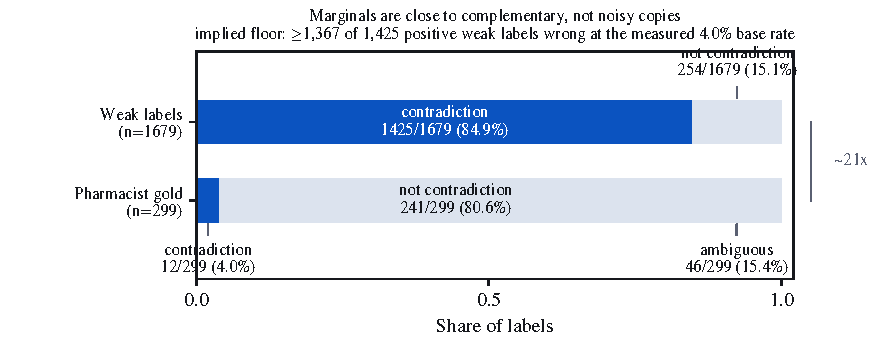
\includegraphics[width=0.92\linewidth]{figures/fig-prevalence.pdf}
\caption{The prevalence mismatch. The reader should notice that the two
distributions are not noisy versions of each other; they are close to
complementary. No aggregation or noise-robust loss recovers a correct
conditional from supervision whose marginal is inverted.}
\label{fig:prevalence}
\end{figure}

\begin{figure}[t]
\centering
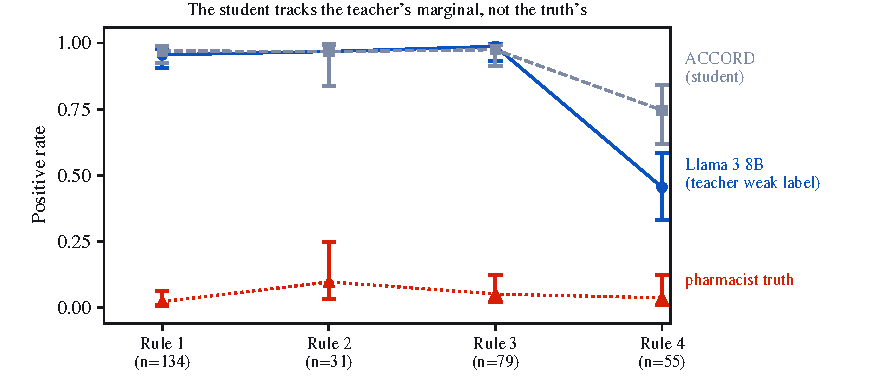
\includegraphics[width=0.92\linewidth]{figures/fig-tracking.pdf}
\caption{Marginal transfer from teacher to student. On Rules 1 to 3 the student's
positive rate is within $1.5$ points of the teacher's while true prevalence
varies fourfold across the same rules. On Rule 4, where the teacher is
genuinely selective, the student regresses towards its own global prior rather
than inheriting the selectivity.}
\label{fig:tracking}
\end{figure}

\section{Limitations}
\label{sec:weak-limitations}

\paragraph{One labeller.} Every conclusion in this chapter concerns Llama 3 8B
under one prompt. Whether a larger model, a different prompt, a chain-of-thought
format, or a calibrated decision rule would behave differently is untested here.
Chapter~\ref{ch:eval} reports a GPT-4o comparison on the gold set only, which is
suggestive but not a weak-supervision experiment.

\paragraph{A related model-agnostic claim in this project is withdrawn.} An
earlier project artifact reported that clinical miscalibration was
``model-agnostic'' on the basis of two models. Only one of the two loaded; the
second returned an authorisation failure on every run, and its row in the
results table was a hardcoded literal. The claim rests on one model and is
retracted. It is mentioned here because the same failure default, scoring
unparseable generations as positive, appears in that component, and is the basis
of the [TODO] in Section~\ref{sec:weak-acquiescence}.

\paragraph{The base rate is measured on $299$ pairs with $12$ positives.} The
$4.0\%$ figure has a wide confidence interval. The $21\times$ ratio would remain
large under any plausible interval, but it should not be quoted to more than one
significant figure.

\paragraph{The exemplar defect confounds the weak labels in the same way it
confounds the gold labels.} The labeller saw the same $41.4\%$-contaminated
exemplars. Unlike the gold labels, however, the weak labels are not used as
ground truth anywhere in this thesis; they are used only as training
supervision, and the claim made about them, that their marginal is wrong by
$21\times$, does not depend on which sentences were shown.

\paragraph{No attempt was made to correct the mismatch.} Prior correction,
threshold shifting, class-balanced resampling, and positive-unlabelled learning
are all standard responses to a known prior shift, and none was tried. This is a
gap in the work, not evidence that they would have failed.
Chapter~\ref{ch:eval}'s threshold sweep bears on this: the model's scores carry
no ranking signal at all, so post-hoc threshold correction has nothing to work
with. That is an argument that correction would not have sufficed \emph{here},
not that prior correction is generally ineffective.

\section{Summary}
\label{sec:weak-summary}

An instruction-tuned language model labelled $1{,}679$ candidate pairs and
called $84.9\%$ of them contradictions against a measured base rate of $4.0\%$.
At least $95\%$ of its positive labels are false positives. The detector trained
on those labels reproduces the labeller's per-rule positive rate to within
$1.5$ percentage points on three of four rules, while the rules' true
prevalences differ from one another by more than a factor of four, which is the
signature of a model that has learned the label's marginal rather than its
conditional. On the one rule where the labeller was genuinely selective, the
student regressed towards its own prior instead of inheriting the distinction.

The confidence field accompanying the weak labels takes two values and is a
deterministic function of the label. It was used both as a filter, where it
removed nothing, and as a per-example loss weight, where it silently reweighted
by class.

The whole failure is detectable before training, with a base-rate estimate, a
printed marginal, a distinct-value count, and a direct comparison against the
human labels that were already available. Chapter~\ref{ch:arch} turns to the
model that consumed these labels, and to three architectural claims that do not
survive contact with the code that produced them.
